\documentclass[10pt]{jarticle}
\usepackage{float}
\usepackage{adrobo_abst}
\usepackage[dvipdfmx]{graphicx}
\usepackage{amssymb,amsmath}
\usepackage{bm}
\usepackage[superscript]{cite}
\usepackage{enumerate}
\usepackage{url}
\usepackage{here}
%\usepackage[absolute]{textpos}
\usepackage{setspace}

\renewcommand\citeform[1]{(#1)}

\begin{document}
%\setstretch{0.90}
    
    \makeatletter
    \doctype{2023年度卒業論文概要}
    \title{自律移動ロボットのためのYOLOv5を用いた\\AutoMSRCR画像からの水たまり検出}{}
    \etitle{Puddle detection from AutoMSRCR images using YOLOv5 \\for autonomous mobile robots}{}
    
    \author{20C1106\hspace{.5zw}松井大和}
    \eauthor{Yamato Matsui}
    
    \makeatother
    
    \abstract{We tested the effectiveness of the AutoMSRCR-based puddle detection method in an environment where mobile robots run.
    In a previous study, the contrast of puddles was enhanced by applying AutoMSRCR to camera images.
    The enhanced images are then trained using YOLO, and the improvement in puddle detection performance is confirmed.
    However, this was only verified in a natural environment where overexposure occurred.
    The detection performance in environments on paved road surfaces or in environments where reflection of scenery is likely to occur has not yet been verified.
    Therefore, we evaluated this method in such environments.}
    
    \keywords{Mechanical Engineering, Keywords List}
    
    \maketitle
    
    \supervisor{指導教員:上田隆一 准教授}
    
    \section{緒\hspace{2zw}言}%===========================
    
    近年, 日本では労働人口の減少が問題となっており, 
    その解決のため自律移動ロボットの利用が試みられている. 
    自律移動ロボットを施設の清掃や警備, 荷物の運搬などに利用するためには
    様々な技術が求められる. 
    特に障害物回避はロボットや環境の保護のために不可欠な技術であり, 
    これまで主に立体的な障害物を対象に研究開発が進められてきた\cite{朝田2019} . 
    しかしながら, 屋外には水たまりをはじめとする平面的な障害物も存在し, 
    それらの回避も求められる場合がある. ロボットが水たまり上を走行すると, 
    浸水による故障, 窪みによるスタックやオドメトリの誤差の増加, 
    水の飛散による周囲の人への被害などを及ぼすことが予測される. 
    したがって屋外自律移動ロボットには水たまりを検出し回避することが, 
    重要な課題となる.\\ 
     しかし, 水たまりは不規則な形状であることや景色の映り込みが発生しやすい性質から, 
    検出が困難である. そのため形状や反射光に左右されない検出手法が求められる.\\
      水たまり検出に関する取り組みとして, 
    色調を調整したカメラ画像からYOLOを用いて水たまりを検出した研究事例がある. 
    Xiaodongら\cite{Xiaodong2022}はカメラ画像からの水たまり検出が困難である要因が水の性質による
    低コントラスト化にあると考え, カメラ画像に処理をかけ水のコントラストを強化する手法を提案した. 
    この研究では複数の画像処理手法の比較検証をおこなった. 
    その結果, AutoMSRCRという環境光の影響を低減し物体の色を復元する処理を施した画像を学習させたモデルで
    水たまりの検出性能の向上を確認している. 
    しかし, この研究では露出オーバーの発生した自然環境でのみ検証された.  
    そのため自律移動ロボットが走行するような環境において, 有効性の確認がされていない.   \\
     そこで本研究では, AutoMSRCR処理を用いた水たまり検出手法の, 移動ロボットを動かす環境への応用を目的とする. 
    舗装された路面上や映り込みが発生しやすい環境の水たまりにおいての本手法
    の有効性を検証する.


    \section{手法}%===========================
        XiaodongらのAutoMSRCR処理を用いた水たまり検出手法について述べる. 
    以下がXiaodongらの研究で用いたデータセットの作成と学習の手順である. 
    \begin{quote}
        \begin{enumerate}
         \item 水たまりを含む画像の撮影
         \item 撮影した画像にAutoMSRCR処理
         \item 水たまり部分をアノテーション
         \item YOLOを用いて学習
        \end{enumerate}
       \end{quote}
     自律移動ロボットが走行する環境を想定し, 
    映り込みの多い環境や舗装された路面の水たまりを中心に撮影する. 今回は651枚の画像を用意した. 
    撮影した画像に対しAutoMSRCR処理を適用する. 
    \begin{figure}[H]
        \begin{tabular}{cc}
            \begin{minipage}{.1\textwidth}
                \centering
                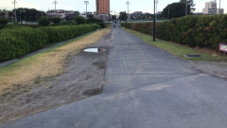
\includegraphics[width=2.0\linewidth]{./fig/fig1.png}
                \vspace{-10mm}\caption{Original}
                \label{fig_first}
            \end{minipage}
            \begin{minipage}{.5\textwidth}
                \centering
                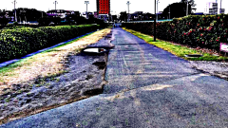
\includegraphics[width=0.4\linewidth]{./fig/fig2.png}
                \vspace{-5mm}\caption{AutoMSRCR}
                \label{fig_second}
            \end{minipage}
        \end{tabular}
    \end{figure}
    その際データセット作成に使用する画像と推定に用いる画像の両方に適用する. 
    アノテーションツールにはVoTTを使用し, 1クラスのみでタグ付けを行う. 
    このようにして作成したデータセットをYOLOv5を用いて学習する. 


    \section{実験}%===========================
    舗装された路面上や映り込みが発生しやすい環境でのAutoMSRCR画像からの水たまり検出手法
    の有効性を検証する. 
    評価のため用意した水たまりを含む画像から10枚を抽出し, 
    オリジナル画像の学習モデルとAutoMSRCR画像の学習モデルのそれぞれを使用して推定, 評価をする. \\
     評価基準は以下のものとする. 
    \begin{quote}
        \begin{itemize}
         \item Recall(R) 
         \item Precision(P) 
         \item しきい値をIoU: 0.5とする
         \item RとP両方の値が1.0だった場合をTrue(T), 
         そうでない場合をFalse(F)とする
         
        \end{itemize}
       \end{quote}
     検証の結果, オリジナル画像の学習モデル(表1)は検出率が4/10であったのに対し, 
    AutoMSRCR画像の学習モデル(表2)では検出率が6/10であった. 
    %このことから舗装された路面上や映り込みが発生しやすい環境においてもこの手法は有効であると言える. 

    \section{結言}%===========================
    本稿では, 舗装された路面上や映り込みが発生しやすい環境でのAutoMSRCR画像からの水たまり検出手法
    の有効性を検証した. 検証の結果, オリジナル画像の学習モデルに比べAutoMSRCR画像の学習モデルでは
    水たまりのみを検出できた割合が2割向上した可能性が高い. 
    %そのため自律移動ロボットが走行する環境においても本手法が有効であるといえる.
     


    



    
    
 
    \vspace{5truemm}
    {\footnotesize
        \begin{thebibliography}{99}

            \bibitem{朝田2019}
            朝田諒, 飯田訓久, 村主勝彦, 増田良平: ``ロボットコンバインのためのステレオカメラを用いた
            物体検出および衝突回避'',農業食料工学会誌, 81 (2019), pp. 392-402.

            \bibitem{Xiaodong2022}
            Xiaodong Guo: ``Research on Water Hazards Detection Method Based on A-MSRCR and Improved YOLO, ''
            Proceedings of the 2022 IEEE International Conference on Robotics and Biomimetics, 
            December 5-9, (2022). 

            
            
        \end{thebibliography}
    }
    \normalsize



    \begin{table}[H]
        \caption{Original model}
        \begin{tabular}{|l|l|l|l|l|l|}
        \hline
           & Answer & Result & R   & P   & T or F \\ \hline
        1  & \begin{minipage}{.1\textwidth}
            \centering
            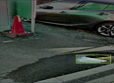
\includegraphics[width=0.9\linewidth]{./fig/tab1_a.png}
        \end{minipage}       & \begin{minipage}{.1\textwidth}
            \centering
            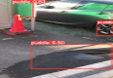
\includegraphics[width=0.9\linewidth]{./fig/tab1_r.png}
           \end{minipage}       & 0.0 & 0.0 & F     \\ \hline
        2  & \begin{minipage}{.1\textwidth}
            \centering
            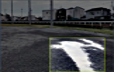
\includegraphics[width=0.9\linewidth]{./fig/tab2_a.png}
           \end{minipage}       & \begin{minipage}{.1\textwidth}
            \centering
            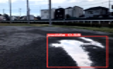
\includegraphics[width=0.9\linewidth]{./fig/tab2_r.png}
           \end{minipage}       & 1.0 & 1.0 & T       \\ \hline
        3  & \begin{minipage}{.1\textwidth}
            \centering
            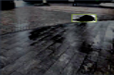
\includegraphics[width=0.9\linewidth]{./fig/tab3_a.png}
           \end{minipage}       & \begin{minipage}{.1\textwidth}
            \centering
            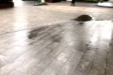
\includegraphics[width=0.9\linewidth]{./fig/tab3_r.png}
           \end{minipage}       & 0.0 & 0.0 & F      \\ \hline
        4  & \begin{minipage}{.1\textwidth}
            \centering
            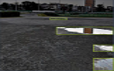
\includegraphics[width=0.9\linewidth]{./fig/tab4_a.png}
           \end{minipage}       & \begin{minipage}{.1\textwidth}
            \centering
            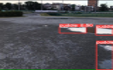
\includegraphics[width=0.9\linewidth]{./fig/tab4_r.png}
           \end{minipage}       & 0.0 & 0.0 & F      \\ \hline
        5  & \begin{minipage}{.1\textwidth}
            \centering
            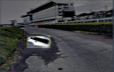
\includegraphics[width=0.9\linewidth]{./fig/tab5_a.png}
           \end{minipage}       & \begin{minipage}{.1\textwidth}
            \centering
            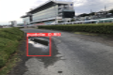
\includegraphics[width=0.9\linewidth]{./fig/tab5_r.png}
           \end{minipage}       & 1.0 & 1.0 & T       \\ \hline
        6  & \begin{minipage}{.1\textwidth}
            \centering
            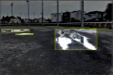
\includegraphics[width=0.9\linewidth]{./fig/tab6_a.png}
           \end{minipage}       & \begin{minipage}{.1\textwidth}
            \centering
            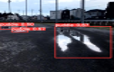
\includegraphics[width=0.9\linewidth]{./fig/tab6_r.png}
           \end{minipage}       & 0.0 & 0.0 & F      \\ \hline
        7  & \begin{minipage}{.1\textwidth}
            \centering
            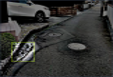
\includegraphics[width=0.9\linewidth]{./fig/tab7_a.png}
           \end{minipage}       & \begin{minipage}{.1\textwidth}
            \centering
            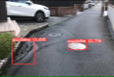
\includegraphics[width=0.9\linewidth]{./fig/tab7_r.png}
           \end{minipage}       & 1.0 & 0.5 & F      \\ \hline
        8  & \begin{minipage}{.1\textwidth}
            \centering
            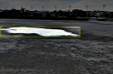
\includegraphics[width=0.9\linewidth]{./fig/tab8_a.png}
           \end{minipage}       & \begin{minipage}{.1\textwidth}
            \centering
            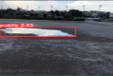
\includegraphics[width=0.9\linewidth]{./fig/tab8_r.png}
           \end{minipage}       & 1.0 & 1.0 & T       \\ \hline
        9  & \begin{minipage}{.1\textwidth}
            \centering
            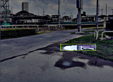
\includegraphics[width=0.9\linewidth]{./fig/tab9_a.png}
           \end{minipage}       & \begin{minipage}{.1\textwidth}
            \centering
            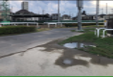
\includegraphics[width=0.9\linewidth]{./fig/tab9_r.png}
           \end{minipage}       & 0.0 & 0.0 & F      \\ \hline
        10 & \begin{minipage}{.1\textwidth}
            \centering
            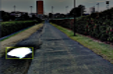
\includegraphics[width=0.9\linewidth]{./fig/tab10_a.png}
           \end{minipage}       & \begin{minipage}{.1\textwidth}
            \centering
            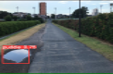
\includegraphics[width=0.9\linewidth]{./fig/tab10_r.png}
           \end{minipage}       & 1.0 & 1.0 & T      \\ \hline
        \end{tabular}
        \end{table}


    \begin{table}[H]
        \caption{AutoMSRCR model}
        \begin{tabular}{|l|l|l|l|l|l|}
        \hline
           & Answer & Result & R   & P   & T or F \\ \hline
        1  & \begin{minipage}{.1\textwidth}
            \centering
            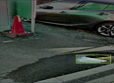
\includegraphics[width=0.9\linewidth]{./fig/2tab1_a.png}
        \end{minipage}       & \begin{minipage}{.1\textwidth}
            \centering
            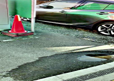
\includegraphics[width=0.9\linewidth]{./fig/2tab1_r.png}
           \end{minipage}       & 0.0 & 0.0 & F      \\ \hline
        2  & \begin{minipage}{.1\textwidth}
            \centering
            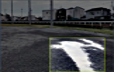
\includegraphics[width=0.9\linewidth]{./fig/2tab2_a.png}
           \end{minipage}       & \begin{minipage}{.1\textwidth}
            \centering
            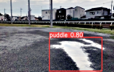
\includegraphics[width=0.9\linewidth]{./fig/2tab2_r.png}
           \end{minipage}       & 1.0 & 1.0 & T       \\ \hline
        3  & \begin{minipage}{.1\textwidth}
            \centering
            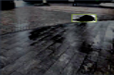
\includegraphics[width=0.9\linewidth]{./fig/2tab3_a.png}
           \end{minipage}       & \begin{minipage}{.1\textwidth}
            \centering
            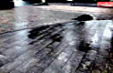
\includegraphics[width=0.9\linewidth]{./fig/2tab3_r.png}
           \end{minipage}       & 0.0 & 0.0 & F      \\ \hline
        4  & \begin{minipage}{.1\textwidth}
            \centering
            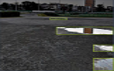
\includegraphics[width=0.9\linewidth]{./fig/2tab4_a.png}
           \end{minipage}       & \begin{minipage}{.1\textwidth}
            \centering
            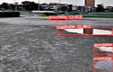
\includegraphics[width=0.9\linewidth]{./fig/2tab4_r.png}
           \end{minipage}       & 0.0 & 0.0 & F      \\ \hline
        5  & \begin{minipage}{.1\textwidth}
            \centering
            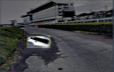
\includegraphics[width=0.9\linewidth]{./fig/2tab5_a.png}
           \end{minipage}       & \begin{minipage}{.1\textwidth}
            \centering
            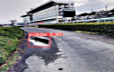
\includegraphics[width=0.9\linewidth]{./fig/2tab5_r.png}
           \end{minipage}       & 1.0 & 1.0 & T       \\ \hline
        6  & \begin{minipage}{.1\textwidth}
            \centering
            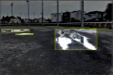
\includegraphics[width=0.9\linewidth]{./fig/2tab6_a.png}
           \end{minipage}       & \begin{minipage}{.1\textwidth}
            \centering
            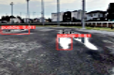
\includegraphics[width=0.9\linewidth]{./fig/2tab6_r.png}
           \end{minipage}       & 0.0 & 0.0 & F      \\ \hline
        7  & \begin{minipage}{.1\textwidth}
            \centering
            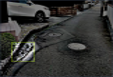
\includegraphics[width=0.9\linewidth]{./fig/2tab7_a.png}
           \end{minipage}       & \begin{minipage}{.1\textwidth}
            \centering
            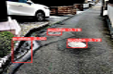
\includegraphics[width=0.9\linewidth]{./fig/2tab7_r.png}
           \end{minipage}       & 1.0 & 0.5 & F      \\ \hline
        8  & \begin{minipage}{.1\textwidth}
            \centering
            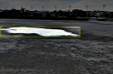
\includegraphics[width=0.9\linewidth]{./fig/2tab8_a.png}
           \end{minipage}       & \begin{minipage}{.1\textwidth}
            \centering
            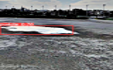
\includegraphics[width=0.9\linewidth]{./fig/2tab8_r.png}
           \end{minipage}       & 1.0 & 1.0 & T       \\ \hline
        9  & \begin{minipage}{.1\textwidth}
            \centering
            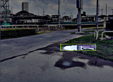
\includegraphics[width=0.9\linewidth]{./fig/2tab9_a.png}
           \end{minipage}       & \begin{minipage}{.1\textwidth}
            \centering
            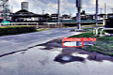
\includegraphics[width=0.9\linewidth]{./fig/2tab9_r.png}
           \end{minipage}       & 0.0 & 0.0 & F      \\ \hline
        10 & \begin{minipage}{.1\textwidth}
            \centering
            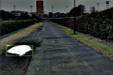
\includegraphics[width=0.9\linewidth]{./fig/2tab10_a.png}
           \end{minipage}       & \begin{minipage}{.1\textwidth}
            \centering
            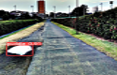
\includegraphics[width=0.9\linewidth]{./fig/2tab10_r.png}
           \end{minipage}       & 1.0 & 1.0 & T      \\ \hline
        \end{tabular}
        \end{table}
 


    
\end{document}
